\documentclass[aps,prl,twocolumn,superscriptaddress,nofootinbib]{revtex4-2}
\usepackage{amsmath,amssymb,amsfonts}
\usepackage{graphicx}
\usepackage{hyperref}
\usepackage{siunitx}
\usepackage{booktabs}

% Auto-generated by update_counts.py — 2026-10-14T09:43:30.211762
% Do not edit manually. Run: uv run python scripts/update_counts.py
\newcommand{\leantoolchain}{4.32.0}
\newcommand{\mathlibrev}{81a5d257}
\newcommand{\physlibrev}{c4843367}
\newcommand{\totaltheorems}{26353}
\newcommand{\substantivetheorems}{26327}
\newcommand{\placeholdertheorems}{26}
\newcommand{\kernelsubstantivetheorems}{26258}
\newcommand{\trackedvacuitydebt}{69}
\newcommand{\axiomcount}{0}
\newcommand{\sorrycount}{0}
\newcommand{\sorrypercent}{0.0}
\newcommand{\leanmodules}{2101}
\newcommand{\leandefinitions}{14045}
\newcommand{\pythonmodules}{138}
\newcommand{\testfiles}{214}
\newcommand{\totaltests}{7673}
\newcommand{\figurecount}{170}
\newcommand{\notebookcount}{91}
\newcommand{\papercount}{42}
\newcommand{\aristotleproved}{313}
\newcommand{\aristotleruns}{40}
% --- D11 bundle substrate summary (source-level, stated rule) ---
\newcommand{\dxiModules}{22}
\newcommand{\dxiLines}{6267}
\newcommand{\dxiTheorems}{403}
\newcommand{\dxiDefs}{82}
\newcommand{\dxiDepsTheorems}{409}
% --- Paper 18 / Phase 5t per-section counts (FermiHubbardDimer.lean) ---
\newcommand{\fhdTotal}{130}
\newcommand{\fhdWaveTwo}{13}
\newcommand{\fhdWaveThree}{6}
\newcommand{\fhdWaveFour}{19}
\newcommand{\fhdWaveFive}{20}
\newcommand{\fhdWaveSixABC}{35}
\newcommand{\fhdWaveSixExtra}{13}
\newcommand{\fhdWaveSeven}{17}
\newcommand{\fhdWaveEight}{7}
% --- Paper 26 / 27 per-module counts (BH entropy + four laws) ---
\newcommand{\bhEntropyTotal}{32}
\newcommand{\bhThermoTotal}{20}
% --- Phase 6 per-module + pytest counts (paper32 / paper34-38 / note_rt_ch_bounds) ---
\newcommand{\strongCpDeThms}{8}
\newcommand{\strongCpDeTests}{14}
\newcommand{\epThms}{24}
\newcommand{\epTests}{38}
\newcommand{\qecHolographyThms}{10}
\newcommand{\qecHolographyTests}{30}
\newcommand{\centerSymmThms}{18}
\newcommand{\centerSymmTests}{28}
\newcommand{\chiralSsbThms}{10}
\newcommand{\chiralSsbTests}{14}
\newcommand{\cflThms}{12}
\newcommand{\cflTests}{17}
\newcommand{\rtChThms}{7}
\newcommand{\rtChTests}{29}
\newcommand{\heatKernelThms}{20}
\newcommand{\heatKernelTests}{39}
\newcommand{\higherCurvatureThms}{13}
\newcommand{\higherCurvatureTests}{42}
\newcommand{\diffInvarianceThms}{13}
\newcommand{\diffInvarianceTests}{36}
\newcommand{\nonlinearEFEThms}{13}
\newcommand{\nonlinearEFETests}{40}
\newcommand{\microscopicCoefficientMatchThms}{12}
\newcommand{\microscopicCoefficientMatchTests}{42}
\newcommand{\einsteinCartanExtensionThms}{12}
\newcommand{\einsteinCartanExtensionTests}{41}
\newcommand{\bbnThms}{14}
\newcommand{\bbnTests}{16}
% --- Phase 6f/6g classical-GR per-module + wave totals (I1 §11–§13) ---
\newcommand{\curvatureThms}{14}
\newcommand{\einsteinTensorThms}{9}
\newcommand{\energyConditionsThms}{8}
\newcommand{\exactSolutionsThms}{16}
\newcommand{\admFormalismThms}{10}
\newcommand{\tetradFormalismThms}{5}
\newcommand{\phaseSixfWonesixTotal}{62}
\newcommand{\phaseSixfWsevenTotal}{13}
\newcommand{\riemannCoordinateThms}{8}
\newcommand{\riemannDifferentialBianchiThms}{8}
\newcommand{\bundleRiemannAuxThms}{6}
\newcommand{\bundleRiemannThms}{7}
\newcommand{\leviCivitaThms}{7}
\newcommand{\phaseSixfWeightTotal}{36}
\newcommand{\riccatiComparisonThms}{11}
\newcommand{\mazurSigmaModelRigidityThms}{12}
\newcommand{\hawkingPenroseCurveThms}{6}
\newcommand{\areaTheoremCurveThms}{10}
\newcommand{\phaseSixgWnineTotal}{39}
% --- D2 chirality-bundle per-module theorem counts (same convention as \totaltheorems) ---
\newcommand{\dtwoSmFermionDataThms}{19}
\newcommand{\dtwoZsixteenAnomalyThms}{23}
\newcommand{\dtwoVecGMonoidalThms}{11}
\newcommand{\dtwoToricCodeCenterThms}{25}
\newcommand{\dtwoCenterEquivalenceThms}{10}
\newcommand{\dtwoGoltermanShamirThms}{32}
\newcommand{\dtwoLatticeHamiltonianThms}{33}
\newcommand{\dtwoTpfEvasionThms}{14}
\newcommand{\dtwoPauliMatricesThms}{15}
\newcommand{\dtwoBdgHamiltonianThms}{8}
\newcommand{\dtwoChiralityWallMasterThms}{16}
\newcommand{\dtwoOnsagerAlgebraThms}{41}
\newcommand{\dtwoOnsagerContractionThms}{12}
\newcommand{\dtwoGtWeylDoubletThms}{15}
\newcommand{\dtwoFkGappedInterfaceThms}{12}
% --- paper10 per-module theorem counts (same convention as \totaltheorems) ---
\newcommand{\paperTenWangBridgeThms}{8}
\newcommand{\paperTenModularInvarianceThms}{11}
% --- Cross-platform Lean theorem reuse, 1+1D BEC -> 2+1D graphene (D1) ---
% Owner: scripts/count_theorem_reuse.py (population = the nine
% 1+1D BEC modules; REUSED = statement is platform-parametric).
\newcommand{\reuseTransferred}{107}
\newcommand{\reusePopulation}{120}
\newcommand{\reuseSpecific}{13}
\newcommand{\reusePercent}{89.17}
\newcommand{\reusePercentRounded}{89}
\newcommand{\reuseSpecificPercentRounded}{11}


%% Bundle: E2 (tier 4, target PRL | PRR)
%% Source manifest: papers/E2/source_manifest.md
%% Source paper: paper16_graphene_sk_eft (companion content)

%% GENERATED by scripts/render_bundle_counts.py — do not edit.
%% Per-bundle substrate counts, derived from this bundle's declared apex closure
%% (papers/<CODE>/bundle_metadata.json -> apex_theorems -> lean_deps.json).
%% Use these for any statement about THIS paper's verified content.
%% \substantivetheorems in docs/counts.tex is PROJECT-wide; using it for a
%% paper-scoped claim overstates by orders of magnitude (TODO-D9).
%% Closure walks stop at `private` declarations, so these are lower bounds.
\newcommand{\bundleTheorems}{6}
\newcommand{\bundleDecls}{12}
\newcommand{\bundleModules}{6}


\begin{document}

\title{Analog Hawking Radiation in a Bilayer-Graphene de~Laval Nozzle}

\author{J.~Roehm}
\affiliation{Independent Researcher}

\date{\today}

\begin{abstract}
We model analog Hawking current noise in a bilayer-graphene nozzle.
At an assumed gradient $\kappa=\SI{2e12}{\per\second}$, the corrected
illustration gives a low-frequency excess of
\SI{1.2e-26}{\ampere\squared/\hertz}, about $100$ times below the thermal
background. Extracting temperature requires independent transmission,
readout and background calibration. An adopted quadratic dispersive law
gives opposing dispersive and viscous shifts. The law, electrical response,
gradient and transport inputs remain assumptions.
\end{abstract}

\maketitle

%% ══════════════════════════════════════════════════════════════════
\section{Introduction}

A fluid crossing from subsonic to supersonic flow carries a sonic horizon,
which radiates at a temperature fixed by the velocity gradient
there~\cite{Unruh1981,Visser1998,Bilic1999}. Geurs \emph{et
al.}~\cite{Geurs2025} have realized that transition in an electronic fluid:
current through an etched constriction in hBN-encapsulated bilayer graphene
accelerates the electron liquid past its own speed of sound and relaxes it
at a stationary shock. Their sound speed is the Fermi-liquid value
$v_{FL}(n) = \hbar\sqrt{\pi n}/(\sqrt{2}\,m^*) = \SI{440}{\kilo\meter/\second}$
at $n = \SI{e12}{\per\centi\meter\squared}$ [\citenum{Geurs2025}, p.~3],
three orders of magnitude above an atomic Bose--Einstein condensate.
Ref.~\cite{Geurs2025} closes by noting the correspondence and estimating
$T_H \sim \SI{500}{\milli\kelvin}$. What is missing is the observable: the
spectrum, its normalization in a measurable quantity, the corrections to
it, and an account of which inputs are measured and which assumed.

The Hawking temperature is universal,
\begin{equation}
T_H = \frac{\hbar \kappa}{2\pi k_B},
\label{eq:T_H}
\end{equation}
with $\kappa$ the velocity-gradient surface gravity; only $\kappa$
distinguishes platforms. We organize the corrections with the
Schwinger--Keldysh dissipative effective field
theory~\cite{CGL2017a,CGL2017b}, which treats the dispersive and
dissipative channels in one expansion. Two transport inputs enter: Majumdar
\emph{et al.}~\cite{Majumdar2025} report, for ultra-clean monolayer
graphene near charge neutrality, $\sigma_Q \simeq (4\pm1)\,e^2/h$, a
Wiedemann--Franz violation above $200\times$, and a viscosity-to-entropy
ratio within a factor of four of the holographic limit
$\hbar/(4\pi k_B)$~\cite{KSS2005,Romatschke2010}. We adopt these under the
scope conditions below.

%% ══════════════════════════════════════════════════════════════════
\section{Acoustic metric and quasi-1D reduction}

The $2{+}1$D acoustic metric for flow along $x$ is~\cite{Bilic1999}
\begin{equation}
G_{\mu\nu} = \Omega^2
\begin{pmatrix}
-(c_s^2 - v^2)/v_F^2 & -v/v_F^2 & 0 \\
-v/v_F^2 & 1 & 0 \\
0 & 0 & 1
\end{pmatrix}.
\label{eq:metric}
\end{equation}
With translational symmetry along $y$ it block-diagonalizes: the $y$-row
off-diagonals vanish and the $yy$ entry reduces to the conformal factor.
Both are machine-checked in \texttt{DiracFluidMetric.lean} as
\texttt{diracFluidMetric\_y\_offdiag\_zero}
($\forall v, v_F, \Omega^2, j \neq 2: G_{2j} = 0$) and
\texttt{diracFluidMetric\_gyy} ($G_{22} = \Omega^2$), algebraic identities
about Eq.~\eqref{eq:metric} that are exactly what they look like.
The $(t,x)$ block supplies the reduced acoustic geometry; transferring
scattering or readout results additionally requires matching dynamics
and boundary conditions.

The transverse-channel cutoff is the only genuinely $2{+}1$D effect. For a
channel of width $W$ with Dirichlet boundaries,
$\omega_\perp(n) = c_s(n{+}1)\pi/W$. With $W = \SI{1}{\micro\meter}$ and
$c_s = \SI{4.4e5}{\meter/\second}$, $\omega_\perp(0) = \SI{1.38e12}{\per\second}$
exceeds $4\omega_H = \SI{1.27e12}{\per\second}$, leaving the whole
$[0,4\omega_H]$ window single-channel. That inequality is checked in
\texttt{DiracFluidWKB.dean\_lowest\_channel\_above\_four\_omega\_H}, whose
exact content is
$(4.4\!\times\!10^5)\pi/10^{-6} > 4\times3.14\!\times\!10^{11}$: a
comparison of two numerals, with the identification of the left side as
$\omega_\perp(0)$ and the right as $4\omega_H$ carried in prose here rather
than in the theorem, which mentions no device record. The margin is $10\%$;
the factor of four is the separation between $\omega_\perp(0)$ and
$\omega_H$, which is $4.4$. Ref.~\cite{Geurs2025} states no throat width
numerically, remarking only that a momentum-relaxation length
$\sim\SI{2}{\micro\meter}$ is ``comparable to the throat width''
[\citenum{Geurs2025}, p.~6]. Our $W = \SI{1}{\micro\meter}$ sits at the low
end of that, and at $W = \SI{2}{\micro\meter}$ the lowest channel falls to
$2.2\,\omega_H$ and the guarantee fails, so a measured throat width is a
precondition for the quasi-1D treatment rather than a refinement of it.

Finite-width corrections to the greybody factor split into a
surface-gravity term bounded by $(l_{\rm ee}/W)^2$ and evanescent leakage
bounded by $(\omega/\omega_\perp)^2 e^{-2\pi L/W}$, summing to
$\approx 1.8\%$ at $\omega_H$ for the geometry above.
\texttt{QuasiOneDReduction.quasi1D\_validity\_bound} combines them by
triangle inequality and \emph{takes each component bound as a hypothesis};
the underlying analysis, that transverse averaging and sub-cutoff Helmholtz
decay produce these forms, is not proved there.

%% ══════════════════════════════════════════════════════════════════
\section{The horizon gradient scale}

\begin{figure}[t]
\centering
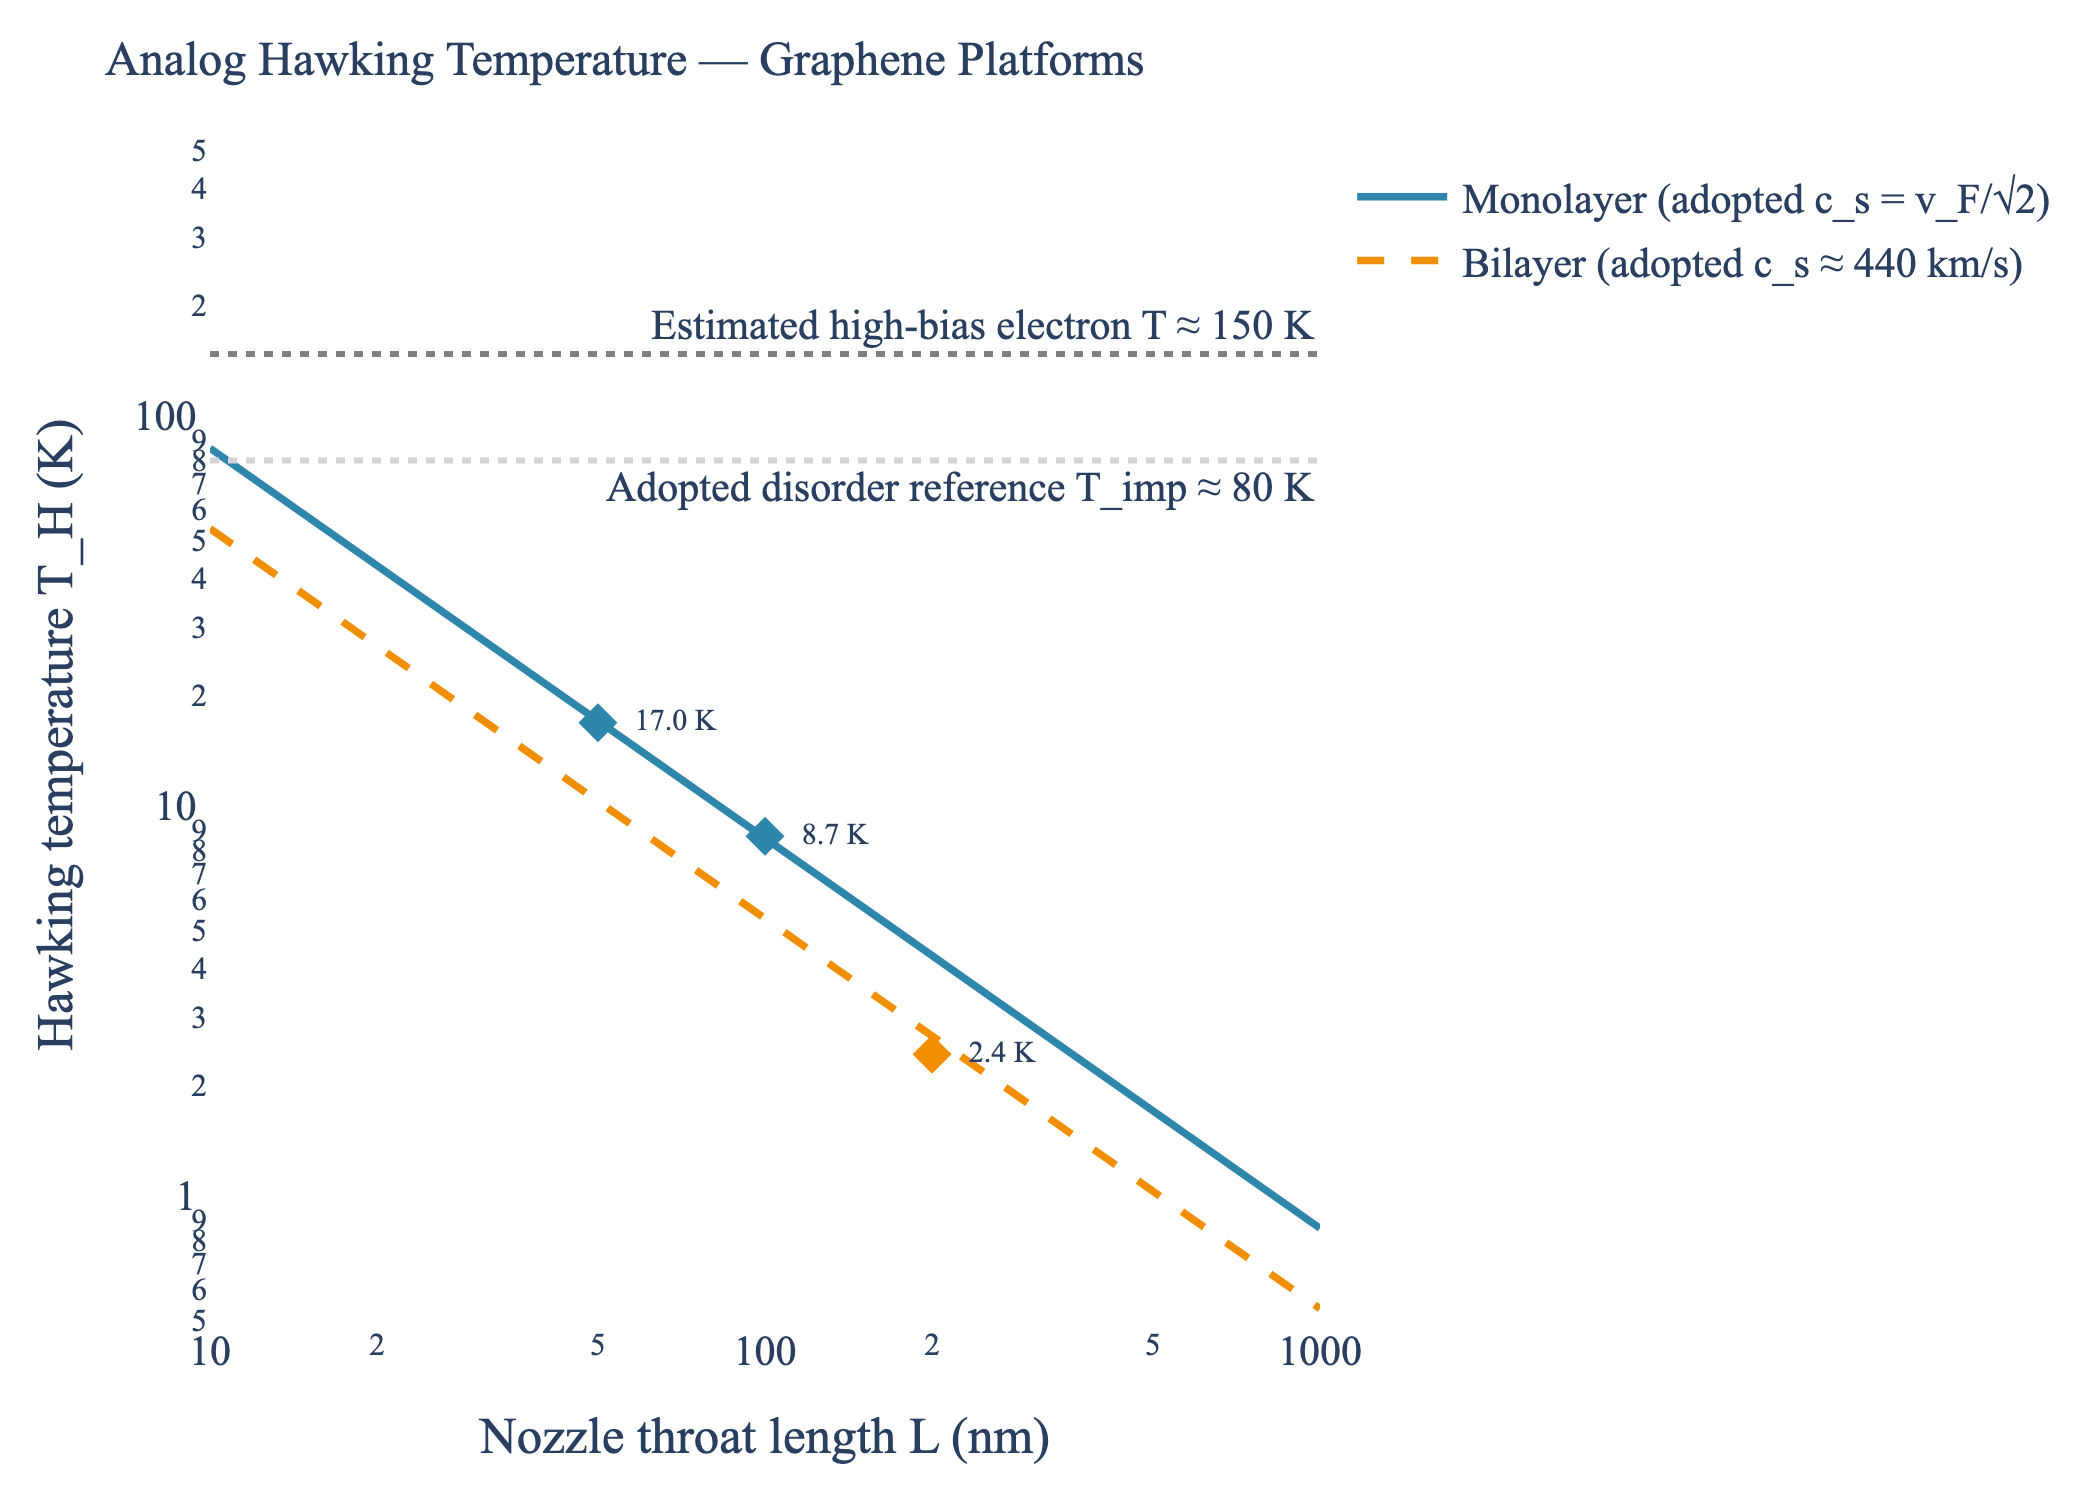
\includegraphics[width=\columnwidth]{figures/fig102_graphene_hawking_T_sweep.png}
\caption{$T_H = \hbar\kappa/2\pi k_B$ versus horizon velocity-gradient
length $L$, with $\kappa = c_s/L$, for the bilayer sound speed
\SI{440}{\kilo\meter/\second} (dashed) and monolayer
\SI{710}{\kilo\meter/\second} (solid). The bilayer point at
$L = \SI{200}{\nano\meter}$ is the assumed gradient of this Letter, not a
measured device dimension. Monolayer points show $T_H$ only and are not
viable operating points: their viscous windows $\omega_H/\Gamma_H$ are
$0.46$ and $0.23$, below unity. Lines: high-bias electron temperature
$T_{\rm e} = \SI{150}{\kelvin}$ [\citenum{Geurs2025}, p.~3] and disorder
scale $T_{\rm imp} \approx \SI{80}{\kelvin}$.}
\label{fig:T_sweep}
\end{figure}

Everything below is proportional to $\kappa$, which is not measured in
Ref.~\cite{Geurs2025}. We take $\kappa = \SI{2.0e12}{\per\second}$,
corresponding through $\kappa \approx c_s/L$ to a gradient length
$L \approx \SI{200}{\nano\meter}$. Equation~\eqref{eq:T_H} gives
\begin{equation}
T_H = \SI{2.43}{\kelvin}, \quad
\omega_H \equiv \frac{k_B T_H}{\hbar} = \SI{3.18e11}{\per\second},
\label{eq:T_H_dean}
\end{equation}
that is $\nu_H = \omega_H/2\pi = \SI{50.7}{\giga\hertz}$ as an ordinary
frequency. This is nine orders of magnitude above the atomic-BEC analog
temperature of \SI{0.35}{\nano\kelvin}~\cite{Steinhauer2016,deNova2019} and
sits inside the \SIrange{1}{10}{\kelvin} window where noise spectroscopy is
routine. That advantage survives every caveat below; $L$ does not.
Ref.~\cite{Geurs2025} contains no nozzle length of
\SI{200}{\nano\meter}: its two occurrences of that scale are a high-bias
momentum-relaxation mean free path and the width of the
Kelvin-probe-resolved shock feature [\citenum{Geurs2025}, p.~6], neither
the velocity gradient at the sonic point. Their own
$T_H \sim \SI{500}{\milli\kelvin}$ corresponds through Eq.~\eqref{eq:T_H}
to $\kappa \approx \SI{4.1e11}{\per\second}$ and a gradient length
$\approx\SI{1}{\micro\meter}$, the throat-width scale. The two temperatures
are not a disagreement about physics but two choices of gradient length
differing by five, and the whole spectrum scales with that choice. We quote
Eq.~\eqref{eq:T_H_dean} because it is what the stated $\kappa$ gives, and
treat the gradient length as the most consequential quantity the experiment
could return.

%% ══════════════════════════════════════════════════════════════════
\section{The two leading corrections}

We parameterize the dispersive correction using
$D = \kappa\,l_{\rm ee}/c_s$, with $l_{\rm ee}$ the electron-electron
scattering length at which hydrodynamics gives out, and adopt
$\delta_{\rm disp} = -c_1 D^2$ with $c_1 = \pi/6$.
The whole quadratic law is phenomenological: neither its power nor its
coefficient is derived from this device's dispersion and profile.
This work's positivity result,
\texttt{GrapheneHawking.graphene\_T\_eff\_positive}, states
$\forall T_H, D: 0 < T_H \wedge D^2 < 6/\pi \Rightarrow
0 < T_H(1 - \tfrac{\pi}{6}D^2)$, proved for the particular choice
$c_1 = \pi/6$ with both hypotheses used. This certifies positivity
of the defined temperature, not the physical ansatz. The pipeline uses
the same canonical $\pi/6$. Changing $c_1$ rescales
the dispersive shifts by $c_1/(\pi/6)$ and can move the crossover with
dissipation or change which contribution dominates.

At the electron temperature $T_{\rm e} = \SI{150}{\kelvin}$ that
Ref.~\cite{Geurs2025} estimates the device reaches under high bias, with
the lattice bath near \SI{10}{\kelvin} [\citenum{Geurs2025}, p.~3], the
framework's $l_{\rm ee} = \hbar v_F/(k_B T)$ evaluates to
\SI{51}{\nano\meter}, giving $D = 0.23$ and
$\delta_{\rm disp} = -2.8\%$ at $c_1 = \pi/6$. Ref.~\cite{Geurs2025},
however, reports $\ell_{\rm ee} \sim \SI{100}{\nano\meter}$ for this
device, as the scale setting the hydraulic-jump width
[\citenum{Geurs2025}, p.~6]; there $D = 0.45$ and
$\delta_{\rm disp} = -11\%$. The discrepancy traces to the Fermi velocity
in $\hbar v_F/(k_B T)$: \SI{e6}{\meter/\second} is the monolayer Dirac
value, whereas the bilayer band is quadratic and the velocity consistent
with the measured $c_s$ is $\sqrt{2}c_s = \SI{6.2e5}{\meter/\second}$.

What the Schwinger--Keldysh damping kernel requires is a
momentum-diffusion constant in \si{\meter\squared\per\second}, not the
relaxation time $\eta/(sT)$:
\begin{equation}
\nu = \frac{\eta\,v_F^2}{w} = 2\,\frac{\eta}{s\,T}\,c_s^2 ,
\label{eq:nu}
\end{equation}
the first equality because relativistic momentum density is $w/v_F^2$, the
second for $c_s^2 = v_F^2/2$. The velocity squared is not decorative:
omitting it turns a time into a dimensionless number and misstates
$\delta_{\rm diss}$ by eleven orders of magnitude. Because the bilayer band
touching is quadratic and admits no emergent light cone, $\nu$ is written
in the \emph{measured} $c_s$ rather than a nominal Fermi velocity. With
$\eta/s = 4\hbar/(4\pi k_B)$ and $T = \SI{150}{\kelvin}$,
$\nu = \SI{6.3e-3}{\meter\squared\per\second}$ and, at $k_H = \kappa/c_s$,
\begin{equation}
\Gamma_H = \nu \left(\frac{\kappa}{c_s}\right)^2
= \SI{1.3e11}{\per\second}, \quad
\delta_{\rm diss} = \frac{\Gamma_H}{\kappa} = +6.5\%.
\label{eq:diss}
\end{equation}
Because $\Gamma_H \propto \kappa^2$ while $\omega_H \propto \kappa$, the
viscous window $\omega_H/\Gamma_H$ shrinks as the horizon steepens, so
narrowing the constriction to raise $T_H$ closes the detection window
rather than opening it.

Within this model, the channels partially cancel, leaving
$T_{\rm eff}/T_H - 1 = +3.7\%$, \emph{above} $T_H$. Small terms
neither establish the leading physical behavior nor bound omitted terms.
For a projected
\SI{100}{\pico\second} cavity at the smooth-horizon parameters of
Falque \emph{et al.}, the same quadratic ansatz gives
$\delta_{\rm disp} \approx -19\%$ against
$\delta_{\rm diss} \approx 14\%$. These comparable values describe
the projection, not the as-built cavity.

The \emph{sign} of the net shift is not yet a prediction. It is $+3.7\%$ at
$l_{\rm ee} = \SI{51}{\nano\meter}$, $c_1 = \pi/6$; $-4.3\%$ at
Ref.~\cite{Geurs2025}'s \SI{100}{\nano\meter}; and $+1.1\%$ at $c_1 = 1$.
These conditional shifts require a measured $l_{\rm ee}$ and a
device-specific dispersive calculation before their sign is a physical
prediction; they supply no general error bound.

Two scope conditions attach to the transport inputs.
Ref.~\cite{Majumdar2025} observes $\sigma_Q \to 4e^2/h$ only for
$|n| \lesssim \SI{5e10}{\per\centi\meter\squared}$ and reports it lower at
larger density [\citenum{Majumdar2025}, p.~5], while the nozzle is quoted
at $n = \SI{e12}{\per\centi\meter\squared}$, twenty times higher; and the
factor-of-four approach to $\hbar/(4\pi k_B)$ holds for the cleanest device
near room temperature, whereas $\eta_{\rm th}/s_{\rm th}$ varies as $1/T^3$
below $T_{\rm imp} \sim \SI{100}{\kelvin}$
[\citenum{Majumdar2025}, p.~7]. Adopting both at
$n = \SI{e12}{\per\centi\meter\squared}$ and \SI{150}{\kelvin} is a
modeling assumption that Ref.~\cite{Majumdar2025}'s own density and
temperature dependence argues against rather than for, and it is
additionally a monolayer-to-bilayer transfer. We use it because no bilayer
measurement exists.

%% ══════════════════════════════════════════════════════════════════
\section{The current-noise observable}

We adopt an electrical-noise response motivated by two analogies:
a modified Callen--Welton fluctuation-dissipation
kernel~\cite{CallenWelton1951}, modeled as $F_u=1+2\Gamma n_H$, and multichannel scattering~\cite{Blanter2000}
with Bogoliubov mixing~\cite{AnantramDatta1996} and
$N_{\rm eff}=\sigma_Qh/(2e^2)$. Assuming this electrical coupling and
channel normalization gives the leading model
\begin{equation}
\boxed{\;\Delta S_I(\omega) = 2\hbar\omega\,\sigma_Q\,\Gamma(\omega)\,n_H(\omega)\;}
\label{eq:noise_psd}
\end{equation}
with $n_H=[e^{\hbar\omega/k_BT_H}-1]^{-1}$ and units
$\mathrm{J}\cdot\mathrm{S}=\mathrm{A}^2/\mathrm{Hz}$.
These analogies do not establish the physical graphene response or the
equivalence of its derivations.
\texttt{GrapheneNoiseFormula.fdt\_consistency} states
$\forall \hbar\omega, \sigma_Q, n_H:
\texttt{hawkingNoisePSD}(\hbar\omega,\sigma_Q,1,n_H)
= 2\hbar\omega\sigma_Q n_H$, the substitution $\Gamma = 1$ into the
definition, discharged by unfolding and ring normalization. It certifies
the closed form's algebraic identity at unit greybody factor. It certifies
neither derivation nor their equivalence, and despite its name no
fluctuation-dissipation content enters it.

For constant $\Gamma$, Eq.~\eqref{eq:noise_psd} has a monotonically
falling Planck shape, $x/(e^x-1)$ with $x=\omega/\omega_H$. Its plateau is
\begin{equation}
\Delta S_I(\omega\to0)=2k_BT_H\sigma_Q\Gamma_0
\simeq\SI{1.0e-26}{\ampere\squared/\hertz},
\label{eq:plateau}
\end{equation}
and its half-height is at $1.6\,\omega_H$ in this leading model.
The corrected numerical illustration below uses a different occupation
and gives approximately \SI{1.2e-26}{\ampere\squared/\hertz}.

Anderson \emph{et al.}~\cite{AndersonBFP2014Graybody}, Eq.~(36), derive
$\Gamma_0=4c_Rv/(c_R+v)^2$ in the infrared for a hydrodynamic,
transversely frozen BEC with stationary constant flow and density and
smooth sound speed approaching fixed asymptotes. Here $c_R$ is the
exterior asymptotic sound speed. Profile independence holds within this
model at $\omega\to0$; it establishes neither graphene transmission nor
finite-frequency behavior. Adopting $c_R\approx c_s$ and $v/c_R=0.985$
gives $\Gamma_0=0.99994$, an illustrative matching assumption.
We also adopt the quadratic roll-off
$\Gamma(\omega)\approx\Gamma_0[1-(\omega/\omega_{\max})^2]$, with
$\omega_{\max}=\sqrt{\kappa c_s/l_{\rm ee}}\approx7.8\,\omega_H$.
This ansatz suppresses transmission by $26.3\%$ at $4\omega_H$; the
cited infrared result supplies no finite-band error bound.

%% ══════════════════════════════════════════════════════════════════
\section{Detection and the falsifiable window}

\begin{figure}[t]
\centering
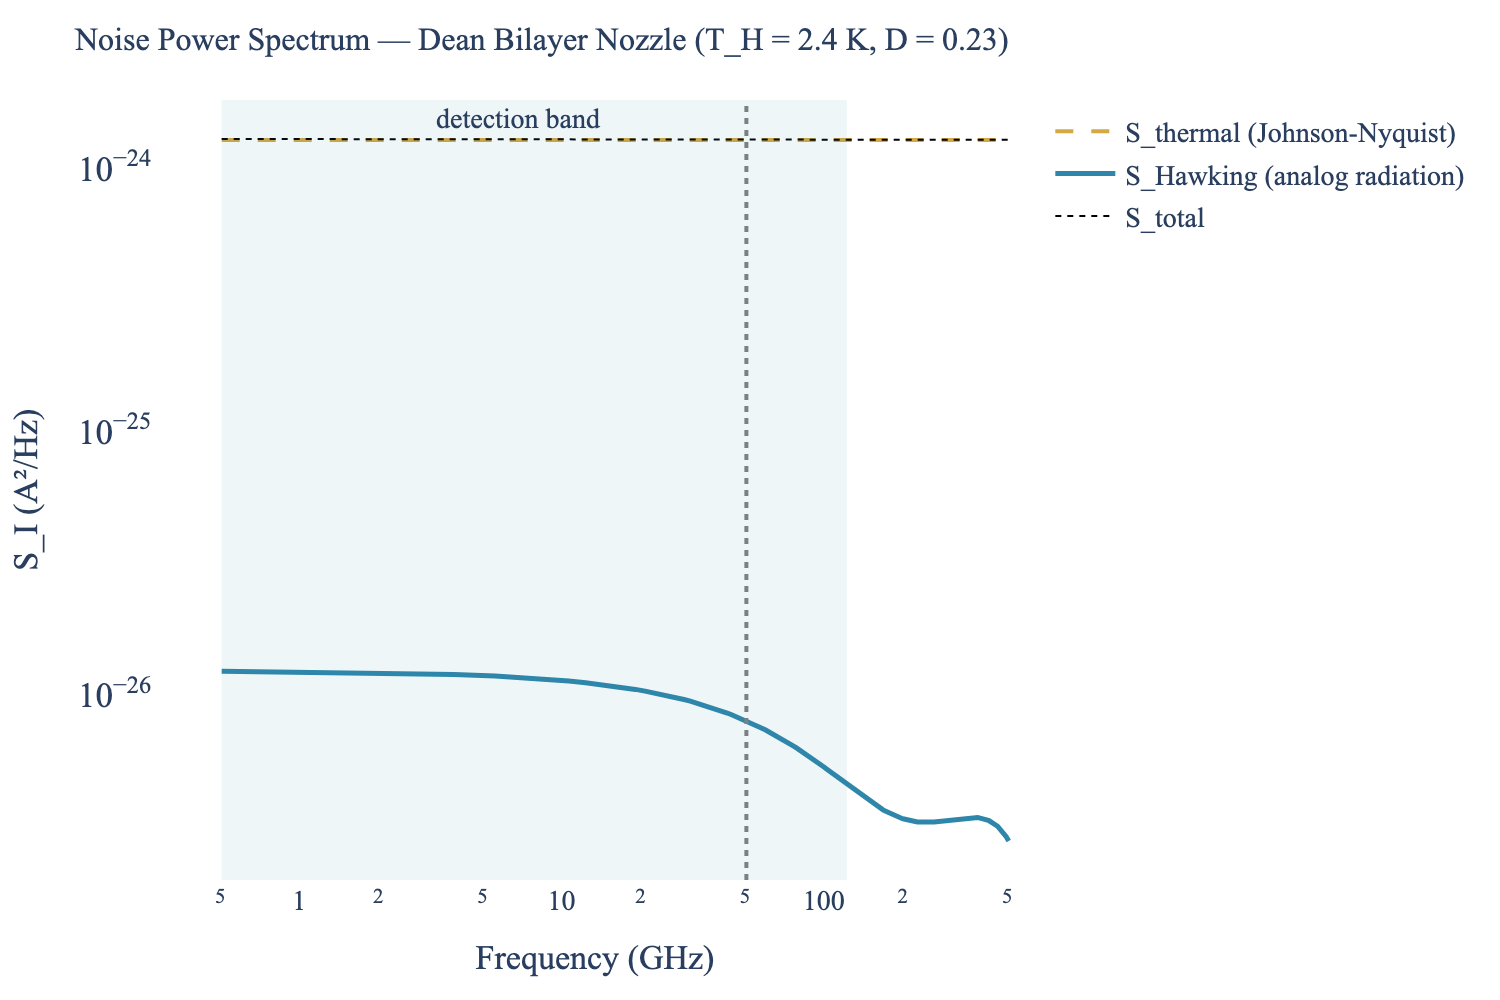
\includegraphics[width=\columnwidth]{figures/fig104_graphene_noise_spectrum.png}
\caption{Adopted corrected noise model at the bilayer-nozzle inputs:
occupation $\beta^2/(1-\delta_K)+n_{\rm noise}$, where $\beta^2$
is the effective-temperature Planck factor, $\delta_K$ the adopted
Keldysh correction and $n_{\rm noise}$ its added floor, with
frequency-dependent greybody transmission. Its low-frequency excess is approximately
\SI{1.2e-26}{\ampere\squared/\hertz}; it is not exactly the leading
Planck model of Eq.~\eqref{eq:noise_psd}. The assumed Johnson--Nyquist
background is $4k_BT_{\rm e}\sigma_Q=\SI{1.3e-24}{\ampere\squared/\hertz}$
at $T_{\rm e}=\SI{150}{\kelvin}$. Shading marks a computed SNR heuristic,
not Eq.~\eqref{eq:falsifiable_window}; extracting a signal requires
transmission, detector-transfer and background calibration.}
\label{fig:noise}
\end{figure}

The corrected illustration has a peak modeled ratio
$S_{\rm Hawking}/S_{\rm thermal}=9.6\times10^{-3}$.
Integrating its squared per-bin ratio across
\SIrange{0.5}{507}{\giga\hertz} gives an ideal statistics-model time of
\SI{1.3e-7}{\second}, or \SI{6.4e-6}{\second} in the single best bin.
These estimates exclude gain drift, background uncertainty and correlated
noise; they establish no achieved sensitivity. Resolving this small
excess requires independent noise and transfer characterization.

We propose the working band
\begin{equation}
\boxed{\;\omega/\omega_H \in [0.5, 4]\;}
\label{eq:falsifiable_window}
\end{equation}
conditionally on measured transmission, dispersion, channel structure and
readout. The low-frequency plateau alone supplies amplitude information;
at the upper edge the adopted roll-off already suppresses $\Gamma$ by
$26.3\%$. The adopted dispersive shift is small at the chosen inputs and
the lowest transverse channel is closed at the assumed $W$; these facts
do not establish a clean, error-controlled detection band.

An unknown $\Gamma(\omega)$, detector transfer or residual background can
alter both shape and normalization. One uncalibrated spectrum therefore
cannot independently identify $T_H$ and $\sigma_Q$; even the leading
plateau determines a product involving $\Gamma_0$ and gain.
With those responses calibrated and operating-point conductivity measured,
a fitted temperature can test Eq.~\eqref{eq:T_H} at a measured velocity
gradient, and normalization can test the adopted noise response.
Disagreement in $T_H$ alone while $\kappa$ is unmeasured is inconclusive.
Required device measurements include the sonic-point gradient, using a
profile technique such as Ref.~\cite{Geurs2025}'s; $\sigma_Q$ and $\eta/s$
at operating density; throat width and electron-electron length at bias;
and independent transmission, electrical-transfer and noise calibration.

Comparison across platforms requires a common normalization, which this
literature does not use uniformly. Falque \emph{et al.}~\cite{Falque2025}
report an exciton-polariton horizon of measured steepness $\kappa = 0.07$
to \SI{0.11}{\per\pico\second} and quote a Hawking temperature of
\SI{3}{\kelvin}. That number is not $\hbar\kappa/2\pi k_B$: their Eq.~(9)
writes the flux as $[e^{\omega/2\pi\kappa}-1]^{-1}$, an exponent smaller
than the standard $2\pi\omega/\kappa$ by $(2\pi)^2$, and it is that
exponent, not its label, which reproduces their quoted fluxes
($I^{\rm HR} = 3$ and $5$ at \SI{20}{\giga\hertz} detuning follow from
their two $\kappa$ to within rounding). Under Eq.~\eqref{eq:T_H} their
$\kappa$ gives \SIrange{0.085}{0.13}{\kelvin}, so Eq.~\eqref{eq:T_H_dean}
sits roughly twenty times above the polariton scale and the apparent
near-agreement is a convention artifact. We compare only at their smooth
horizons: Ref.~\cite{Falque2025} states that their steep-horizon spectrum
is dominated by nonlinear frequency dispersion and is therefore not thermal
[\citenum{Falque2025}, p.~6], and we make no thermal claim about those.

An independent cross-check of the same critical scaling runs through the
Kibble--Zurek--Unruh correspondence, developed with its scope caveat in the
companion paper~\cite{Roehm2026GrapheneDeep}.

%% ══════════════════════════════════════════════════════════════════
\section{Conclusion}

The bilayer-graphene nozzle offers a prospective test of an adopted
Hawking-noise model. The assumed gradient
$\kappa=\SI{2e12}{\per\second}$ gives $T_H=\SI{2.43}{\kelvin}$,
roughly twenty times the smooth polariton scale on a common normalization.
The corrected numerical illustration has a low-frequency excess near
\SI{1.2e-26}{\ampere\squared/\hertz}; its extraction requires calibrated
transmission, electrical response and background. For the adopted
quadratic law and transport inputs, dispersive and dissipative shifts
are comparable, opposite and small. Their ratio and net sign remain
conditional on the law and electron-electron length; a device-specific
dispersive calculation is required.

The unmeasured sonic-point gradient sets the frequency scale and accounts
for the factor-five difference from Ref.~\cite{Geurs2025}'s temperature
estimate. Transport, geometry and readout remain additional experimental
gates. The machine-checked chain
(\texttt{DiracFluidMetric}, \texttt{DiracFluidWKB},
\texttt{GrapheneHawking}, \texttt{GrapheneNoiseFormula},
\texttt{QuasiOneDReduction}; \texttt{lake build} clean, v\leantoolchain,
Mathlib \texttt{\mathlibrev}) supplies the algebraic backbone and none of
the physical inputs, which is why every statement it establishes is quoted
above in full.

\begin{acknowledgments}
Five of the six graphene Dirac-fluid modules are named where their bounds
are used; the sixth, \texttt{DiracFluidSK.lean}, carries the second-order
kernel behind Eq.~\eqref{eq:noise_psd}.
\end{acknowledgments}

\begin{thebibliography}{99}
\bibitem{Roehm2026GrapheneDeep}
J.~Roehm, \emph{Formally Verified Analog Hawking Radiation Across Three
Platforms} (companion paper), in preparation.

\bibitem{Unruh1981}
W.~G.~Unruh, Phys.\ Rev.\ Lett.\ \textbf{46}, 1351 (1981).

\bibitem{Visser1998}
M.~Visser, Class.\ Quant.\ Grav.\ \textbf{15}, 1767 (1998).

\bibitem{Steinhauer2016}
J.~Steinhauer, Nat.\ Phys.\ \textbf{12}, 959 (2016).

\bibitem{deNova2019}
J.~R.~M.~de~Nova \emph{et al.}, Nature \textbf{569}, 688 (2019).

\bibitem{Falque2025}
K.~Falque \emph{et al.}, ``Polariton fluids as quantum field theory
simulators on tailored curved spacetimes,'' Phys.\ Rev.\ Lett.\
\textbf{135}, 023401 (2025) [arXiv:2311.01392].

\bibitem{CGL2017a}
M.~Crossley, P.~Glorioso, and H.~Liu, JHEP \textbf{09}, 095 (2017)
[arXiv:1511.03646].

\bibitem{CGL2017b}
P.~Glorioso, M.~Crossley, and H.~Liu, JHEP \textbf{09}, 096 (2017)
[arXiv:1701.07817].

\bibitem{Geurs2025}
J.~Geurs \emph{et al.}, ``Supersonic flow and hydraulic jump in an
electronic de Laval nozzle,'' arXiv:2509.16321v2 (2025).

\bibitem{Majumdar2025}
A.~Majumdar \emph{et al.}, ``Universality in quantum critical flow of
charge and heat in ultra-clean graphene,'' Nature Physics \textbf{21},
1374 (2025), arXiv:2501.03193.

\bibitem{KSS2005}
P.~K.~Kovtun, D.~T.~Son, and A.~O.~Starinets, Phys.\ Rev.\ Lett.\
\textbf{94}, 111601 (2005).

\bibitem{Bilic1999}
N.~Bili\'c, Class.\ Quant.\ Grav.\ \textbf{16}, 3953 (1999).

\bibitem{Romatschke2010}
P.~Romatschke, Int.\ J.\ Mod.\ Phys.\ E \textbf{19}, 1 (2010).

\bibitem{CallenWelton1951}
H.~B.~Callen and T.~A.~Welton, Phys.\ Rev.\ \textbf{83}, 34 (1951).

\bibitem{AndersonBFP2014Graybody}
P.~R.~Anderson, R.~Balbinot, A.~Fabbri, and R.~Parentani,
``Gray-body factor and infrared divergences in 1D BEC acoustic black holes,''
Phys.\ Rev.\ D \textbf{90}, 104044 (2014), arXiv:1404.3224v3.

\bibitem{Blanter2000}
Ya.~M.~Blanter and M.~B\"uttiker, Phys.\ Rep.\ \textbf{336}, 1 (2000).

\bibitem{AnantramDatta1996}
M.~P.~Anantram and S.~Datta, Phys.\ Rev.\ B \textbf{53}, 16390 (1996).
\end{thebibliography}

\end{document}
